\documentclass{article}
\usepackage[cm]{fullpage}
\usepackage{amsmath}
\usepackage{amssymb}
\usepackage{gensymb}
\usepackage{cancel}
\usepackage[utf8]{inputenc}
\usepackage{verbatim}
\usepackage{tikz}

\usepackage{etoolbox}
\makeatletter
\patchcmd{\@verbatim}
  {\verbatim@font}
  {\verbatim@font\scriptsize}
  {}{}
\makeatother

\usetikzlibrary{calc}

\title{CS 577 HW 7, P2}
\author{William Jen, Matt Henricks}
\date{}

\begin{document}
\maketitle


\begin{enumerate}
    \item[2.]
        \begin{enumerate}
            \item \textbf{Pseudocode}:
        
                \begin{verbatim}
function find_mst(V, E, W):
    if len(E) <= len(V) - 1:
        return # done - already MST 
    
    for i = len(E) .. len(V) - 1:
        init dfs_stack as empty stack
        init visited as empty list
        
        dfs_stack.push(V[1])
        while dfs_stack not empty:
            A = dfs_stack.pop()
            set A as visited
            add A to end of visited list
            
            for each successor s of A:
                if s is not visited:
                    dfs_stack.push(s)
                else:
                    # walk back on the visited list 
                    # look at each pair in the cycle, and pick the two edges
                    # with the biggest weight
                    max_edge_pair = {visited[len(visited)], visited[len(visited) - 1]}
                    i = len(visited) - 1
                    while visited[i] != s:
                        if W[visited[i], visited[i - 1]] > W[max_edge_pair]:
                            max_edge_pair = {visited[i], visited[i - 1]}
                    
                    # check final edge in cycle and compare weights
                    if W[visited[i], visited[len(visited)]] > W[max_edge_pair]:
                        max_edge_pair = {visited[i], visited[len(visited)]}
                    
                    # we have removed something. force dfs to quit early
                    # so that we can restart DFS on the modified graph
                    dfs_stack.clear()
                    break
                \end{verbatim}
            %\clearpage
            \item
                \begin{enumerate}
                    \item \textbf{Counterexample}: Suppose we have a graph:
                        \begin{table}[!h]
                            \centering
                            \begin{tabular}{|c|c|}
                                \hline
                                \textbf{Original Graph} & \textbf{MST} \\ \hline
                                & \\ 
                                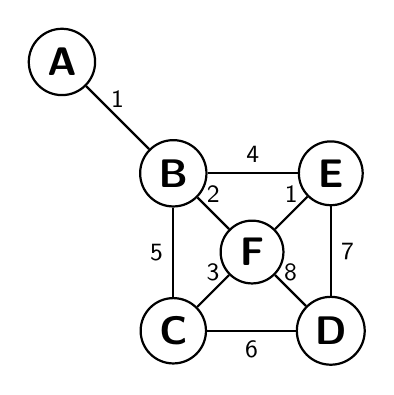
\begin{tikzpicture}[auto, node distance=2cm, every loop/.style={},
                                                    thick,main node/.style={circle,draw,font=\sffamily\Large\bfseries}]
                                    \node[main node] (1) {A};
                                    \node[main node] (2) [below right of=1] {B};
                                    \node[main node] (3) [below of=2] {C};
                                    \node[main node] (4) [right of=3] {D};
                                    \node[main node] (5) [above of=4] {E};
                                    \node[main node] (6) at ($(2)!0.5!(4)$) {F};
                                
                                    \path[every node/.style={font=\sffamily\small}]
                                        (1) edge node [above]  {1} (2)
                                        (2) edge node [above] {4} (5)
                                            edge node [left]  {5} (3)
                                            edge node [above] {2} (6)
                                        (3) edge node [below] {6} (4)
                                            edge node [above] {3} (6)
                                        (4) edge node [right] {7} (5)
                                            edge node [above] {8} (6)
                                        (5) edge node [above] {1} (6);
                                \end{tikzpicture} &
                                
                                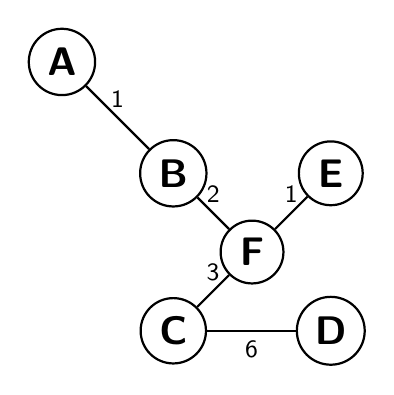
\begin{tikzpicture}[auto, node distance=2cm, every loop/.style={},
                                                    thick,main node/.style={circle,draw,font=\sffamily\Large\bfseries}]
                                    \node[main node] (1) {A};
                                    \node[main node] (2) [below right of=1] {B};
                                    \node[main node] (3) [below of=2] {C};
                                    \node[main node] (4) [right of=3] {D};
                                    \node[main node] (5) [above of=4] {E};
                                    \node[main node] (6) at ($(2)!0.5!(4)$) {F};
                                
                                    \path[every node/.style={font=\sffamily\small}]
                                        (1) edge node [above] {1} (2)
                                        (2) edge node [above] {2} (6)
                                        (3) edge node [below] {6} (4)
                                            edge node [above] {3} (6)
                                        (5) edge node [above] {1} (6);
                                \end{tikzpicture} \\ \hline
                            \end{tabular}
                        \end{table}
                    
                    From this graph, suppose we have a cycle $C = \left\{B, E, D, C \right\}$. The highest
                    cost edge $\epsilon \in C$ is from E to D with a weight of 7. Let's select $\epsilon^\prime$
                    to be the edge from B to C with a cost of 5, and $\epsilon^\prime \not\in T$. The claim
                    is that we can substitute $\epsilon$ for $\epsilon^\prime$ and still arrive at the MST. This
                    is only true iff $\epsilon = \epsilon^\prime$ since as we are supposed to remove the maximum
                    weighted edge on each iteration. However, this is not true, as shown in this example.

                    \item \textbf{Lemma Proof}: For a given $\epsilon \in C$, where the weight of $\epsilon$ is the 
                        max in the cycle, $\epsilon \in T$ or $\epsilon \not\in T$. 
                        \begin{itemize}
                            \item Case $\epsilon \not\in T$: The max edge in the cycle $C$ was removed, and as
                                such there must be a MST contained within the remaining graph $A - 
                                \left\{\epsilon\right\}$.
                            
                            \item Case $\epsilon \in T$: If this is true, there must be a $\epsilon^\prime
                                \not\in E_T$ and is in the cycle $C$. Consequently, $w\left(\epsilon\right)
                                \geq w\left(\epsilon^{\prime}\right)$. If we keep $\epsilon$ and
                                remove $\epsilon^\prime$, we can arrive at another MST via a greedy
                                exchange proof. However, this only holds when $w\left(\epsilon\right) =
                                w\left(\epsilon^\prime\right)$. If they were not the same, removing $
                                \epsilon$ would have made a better MST, which contradicts the given case
                                statement of $\epsilon \in T$.
                        \end{itemize}

                \end{enumerate}
                
            \item 
                \begin{enumerate}
                    \item \textbf{Proof}: We can use a loop invariant to prove the 
                    pseudocode presented in (a). Our loop invariant is that after each
                    iteration $i$, there exists a minimum spanning tree in the modified graph.
                    \item \textbf{Initialization}: $i$ starts at $\text{len}\left(V\right)$.
                    Since we have not removed any edges from the graph, we know that 
                    there exists a minimum spanning tree $T = \left(V, E_T\right)$ for some $E_T \subseteq E$.
                    \item \textbf{Maintenance}: For each iteration, we will search for a cycle in the graph,
                        determine the largest weighted edge in the cycle, and remove it. Note that there exists
                        a cycle in the graph whenever $\text{len}\left(E\right) > \text{len}\left(V\right) - 1$.
                        The loop invariant holds by the lemma proved in part b, part ii.
                    \item \textbf{Termination}: The algorithm will run for exactly $\text{len}\left(E\right) 
                        - \text{len}\left(V\right) - 1$ iterations and remove exactly that number of edges because
                        a minimum spanning tree must have $\text{len}\left(V\right) - 1$ edges.
                \end{enumerate}
            
            \item The algorithm we gave runs in $O\left(EV + E^2\right)$ time in the worst case. The modified DFS
                algorithm runs in $O\left(V + E + V\right) = O\left(E + V\right)$, since on a detection of a cycle 
                requires us to look at all of the vertices that have been visited, and finding the maximum edge weight
                among those vertices. That "walk-back" operation is a $O\left(V\right)$ in the worst case, e.g. our graph
                is an n-gon. In the worst case, we must run DFS on the order of $O\left(E\right)$ iterations.
                
                For the given function $E = n + \sqrt{n}\left(\log n\right)^5$, we can directly compute the number of iterations
                required for our algorithm, which ends up being $\sqrt{n}\left(\log n\right)^5 - 1$. Combining this into the DFS
                time complexity:
                    \begin{flalign*}
                        &= O\left(\sqrt{n}\left(\log n\right)^5 - 1\right) \times O\left(E + V\right) \\
                        &=\left(\sqrt{n}\left(\log n\right)^5\right)\left(\left[n + \sqrt{n}\left(\log n\right)^5\right] + n\right) \\
                        &= n\left(\log n\right)^5\left[\sqrt{n} + \cancel{\left(\log n\right)^5}\right] \\
                        &= O\left(n\sqrt{n}\left(\log n\right)^5\right)
                    \end{flalign*}
                
                Note that $O\left(\sqrt{n}\right) > O\left(\left(\log n\right)^5\right)$, and was removed from the above expression.
                
                We now must examine Kruskal's and Prim's algorithm.
                \begin{itemize}
                    \item \textbf{Kruskal's}:
                        \begin{flalign*}
                            &= O\left(E\log V\right) = \left(n +  \sqrt{n}\left(\log n \right)^5\right)\log n \\
                            &= O\left(n\log n + \sqrt{n}\left(\log n\right)^6\right)
                        \end{flalign*}
                    \item \textbf{Prim's - using fibonacci heap}
                        \begin{flalign*}
                            &= O\left(E + V\log V\right) = \left(n + \sqrt{n}\left(\log n \right)^5\right) + n\log n \\
                            &= O\left(n\log n + n + \sqrt{n}\left(\log n\right)^5\right)
                        \end{flalign*}
                \end{itemize}
                
                It is clear that Prim's MST algorithm is the best out of the algorithms presented.
                
        \end{enumerate}
\end{enumerate}
\end{document}
